
\section{Random variables \skript{25-27}}

\begin{tabular}{p{5.5cm}p{8.5cm}p{4cm}}
$X: \Omega \rightarrow \mathbb{R}$&	$X=\{x_1, \ldots, x_n, \ldots\}$&\\
&&\\
	Discrete random variable (RV): &$P(X=x_i)=P(\{\omega|X(\omega)=x_i\})$& $i=\{1,2,\ldots,n,\ldots\}$\\
	Continuous random variable (RV): &$P(X\in [a,b])=P(\{\omega|X(\omega)=X\in a,b]\})=\int\limits_a^b{f(x)}dx$& $i=[a,b]$ \\
									&																			&$f(x)$: density function.
\end{tabular}

\begin{tabular}{p{5.5cm}p{4cm}p{4cm}}
Normalization:&$\sum\limits_{i=1}^\infty{P(X=x_i)}=1$& $\int\limits_{-\infty}^\infty{f(x)dx}=1$\\
\end{tabular}

\vspace{2mm}
\hrule
\vspace{3mm}

\subsection{Cumulative Distribution Function (Verteilungsfunktion): F(x) \skript{27}}

	\begin{tabular}{p{3cm}p{6cm}}
	
	Discrete: &$F(x)=P(X\leq x)=\sum\limits_{x_i:x_i\leq x}{P(X=x_i)}$\\
	Continuous: &$F(x)=P(X\leq x)=\int\limits_{-\infty}^x{f(x)dx}$\\
	\end{tabular}
	
	\renewcommand{\arraystretch}{1.5}
	\begin{tabular}[]{|l|l|}
	      	\hline
	      	\textbf{Discrete} & \textbf{Continuous}\\
	      	\hline
	      	\hline
	      	$P(X\leq x)=F_X(x)=\sum\limits_{k=-\infty}^x p_k$ &
	      	$P(X\leq x)=F_X(x)=\int\limits_{-\infty}^x
	      	f_X(\tilde{x})d\tilde{x}$\\
				$P(X>x)=1-P(X\leq x)$ & $P(X>x)=1-P(X\leq x)$\\        	
	      	$P(a \le X \leq b)=F_X(b)-F_X(a)=\sum\limits_{k=a}^b p_k$ &
				$P(a \le X \leq b)=F_X(b)-F_X(a)=\int \limits_a^b
				f_X(\tilde{x})d\tilde{x}$\\
	      	\hline
	\end{tabular}
	\renewcommand{\arraystretch}{1}

\subsubsection{Properties}
	$$\boxed{\mathbb{D}(F) = \mathbb{R}} \qquad \boxed{\mathbb{W}(F)
	\in[0,1]} \qquad \boxed{F(-\infty)=0} \qquad  \boxed{F(\infty)=1}
	\qquad \boxed{F(x) \text{ increases monotonically}}$$

\hrule

\vspace{5mm}
	\begin{minipage}{13cm}
	\subsubsection{Probability density function}
		\begin{tabular}{p{3.3cm}p{8.5cm}}
    	$f_X(x)=F'(x)$ & probability density function \\
    	
    	\multirow{2}{11cm}{\textbf{At jump discontinuity of $F_X(x)$: }}\\
    	\multirow{2}{11cm}{$\varphi(x) = $ delta impulse with value of the jump heigh}
    	
    	\end{tabular}
	\end{minipage}
	\begin{minipage}{5cm}
		\subsubsection{Expectation}
			\begin{tabular}{ll}
            $E(X)=\int\limits_{-\infty}^{\infty}{x f_X(x)dx}$\\
        	$E(X^2)=\int\limits_{-\infty}^{\infty}{x^2 f_X(x)dx}$\\
			$E(X^N)=\int\limits_{-\infty}^{\infty}{x^N f_X(x)dx}$\\
        	\end{tabular}
	\end{minipage}
\hrule
\vspace{2mm}

	\subsubsection{Calculation rules for $f_X$ und $F_X$}
		\begin{minipage}{11cm}
			\begin{tabular}{lll}
        	Given: & X, Y Random variables, 
        	&$f_X$, $f_Y$ known\\
        	\end{tabular}\\
 
        	\begin{tabular}{p{6cm}p{6cm}}
        	Probability function: & Density function:\\
        	$F_{X+a}(x)=F_X(x-a)$  &$f_{X+a}(x)=f_X(x-a)$\\
        	$F_{\lambda X}(x)=F_X(\frac{x}{\lambda})$ &$f_{\lambda
        	X}(x)=f_X(\frac{x}{\lambda})\frac{1}{\lambda}$\\
        	$F_{X+Y}(x)=F_X\ast f_Y(y)=F_Y\ast f_X(x)$ &
        	$f_{X+Y}(x)=f_X\ast f_Y(x)$\\
        	$F_{\sqrt{X}}(x)=F_X(x^2)$ &
        	$f_{\sqrt{X}}(x)=2x f_X(x^2)$\\
        	$F_{X^2}(x)=F_X(\sqrt{x})$ &
        	$f_{X^2}(x)=\frac{1}{2}x^{-\frac{1}{2}}f_X(\sqrt{x})$
        	\end{tabular}
		\end{minipage}
		\begin{minipage}{7cm}
        	\subsubsection{Example algorithm}
        	\begin{tabular}{ll}
        	1. Use definition of $F$: $F_{\lambda X}(x)=P(\underbrace
        	{\lambda X\leq x}_{*})$\\[0.5cm]
        	2. Transform * definition: $P(X \leq
        	\frac{x}{\lambda})=F_X(\frac{x}{\lambda})$\\[0.5cm]
        	3. For density: $\frac{d}{dx}$\\[0.5cm]
        	$f_{\lambda X}(x)=\frac{d}{dx}F_{\lambda
        	X}(x)=\frac{d}{dx}F_X(\frac{x}{\lambda})=
        	f_X(\frac{x}{\lambda})\frac{1}{\lambda}$
        	\end{tabular}
			\vspace{10mm}
        \end{minipage}
        
		\subsubsection{Maximum of an interval}
		$X_1,\ldots X_i$ sind auf dem Intervall $[0,l]$ mit $F_X(x)$ verteilt: $M=\max \{ X_1,\ldots,X_i\} $; $F_M(x)=F_X(x)^n$
\vspace{2mm}
\hrule
\vspace{3mm}

\subsection{Expectation: E(x) \skript{28}}
\begin{minipage}{12cm}
  \begin{tabular}{p{2cm}p{4cm}p{5cm} }
  			&  Expectation (1. moment)						&	$n$-th moment	\\
  Discrete:	 &$E(X)=\sum\limits_{i=1}^\infty{x_i P(X=x_i)}$	&	$E(X^n)=\sum\limits_{i=1}^\infty{x_i^n P(X=x_i)}$\\
  Continuous:  &$E(X)=\int\limits_{-\infty}^\infty{x f(x)dx}$	&	$E(X^n)=\int\limits_{-\infty}^\infty{x_i^n f(x)dx}$\\
  \end{tabular}
\end{minipage}
\begin{minipage}{7cm}
  $E(X+Y)=E(X)+E(Y)$\\
  $E(\lambda X + \mu)=\lambda \cdot E(X) + \mu \qquad\lambda, \mu \in \mathbb{R}$\\
  $E(XY) = E(X)\cdot E(Y)$ (if independent)\\
\end{minipage}

\vspace{2mm}
\hrule
\vspace{3mm}

\subsection{Variance: V(X)=Var(X) \skript{28,29}}
  \begin{tabular}{p{2cm}p{8cm}l}
  	$Var(X)$	&	$=E(X^2)-E^2(X)=E\left([X-E(X)]^2\right)$						& \\
  	Discrete: 	&	$V(X)=Var(X)=\sum\limits_{i=1}^\infty{(x_i-E(X))^2 P(X=x_i)}$	& \\
  	Continuous: &	$V(X)=Var(X)=\int\limits_{-\infty}^\infty{(x_i-E(X))^2 f(x)dx}$	& \\
  \end{tabular}

\begin{minipage}{12cm}
    $Var(X+Y)= \begin{cases}
                  Var(X)+Var(Y)
                  & \text{(X,Y independent)}\\                     
                  Var(X) + Var(Y) + 2 \cdot Cov(X,Y) 
                  & \text{(X,Y dependent)}\\
               \end{cases} $ \\
    $Var(X Y)= Var(Y)Var(X)+Var(Y)E(X)^2+Var(X)E(Y)^2$
\end{minipage}
\begin{minipage}{7cm}
    $Var(\lambda X)=\lambda^2 Var(X) \qquad $ $\lambda \in
    \mathbb{R}$\\ 
    $Var(X_1+X_2+\ldots+X_n) \neq Var(n X)$ \\
\end{minipage}
\vspace{2mm}
\hrule
\vspace{3mm}

\subsection{Moment Generating Function $\phi(t)$ \skript{29}}
Used to calculate first or second order moments (mean, variance). If a MGF can be
derived, then the distribution is unique.

\begin{tabular}{p{5cm}p{12cm}}
Discrete: &$\phi(t)=E(\e^{tX})=\sum\limits_{i=1}^\infty{\e^{t x_i} P(X=x_i)}$\\
Continuous: &$\phi(t)=E(\e^{tX})=\int\limits_{-\infty}^\infty{\e^{t x} f(x)dx}$\\
Summation of processes: & $\phi_{X \pm Y}(t) = E(\e^{t(X \pm Y)}) = E(\e^{tX}) E(\e^{t(\pm Y)})=\phi_{X}(t)\cdot\phi_Y(\pm t)$ \\
Example: &$E(X)=\left.\phi'(t)\right|_{t=0} \qquad E(X^2)=\left.\phi''(t)\right|_{t=0} \qquad E(X^n)=\left.\phi^{(n)}(t)\right|_{t=0}$
\end{tabular}

	\vspace{2mm}
	\hrule
	\vspace{3mm}
	

\subsection{Covariance (Abhängigkeit) $Cov(X,Y)$ \skript{40-42}}
\begin{minipage}{12.5cm}
  $Cov(X,Y)=E(XY)-E(X)E(Y)=E([X-E(X)][Y-E(Y)])$ 

  \begin{tabular}{p{2cm}p{9.5cm}}
  Discrete: &$Cov(X,Y)=\sum\limits_{x_i,y_j}{(x_i-E(X))(y_j-E(Y))P({X=x_i,Y=y_i})}$\\
  
  Continuous: &$Cov(X,Y)=\int\limits_{-\infty}^\infty{\int\limits_{-\infty}^\infty{(x-E(X))(y-E(Y))f_{X,Y}(x,y)dy}dx}$\\
  \end{tabular}\\
  
  \textbf{Covariance matrix $P_X$:}\\
  $P_X=\begin{bmatrix}
          Cov(X_1,X_1) & \hdots & Cov(X_1,X_m) \\                                   
          \vdots & \ddots & \vdots \\                             
          Cov(X_m,X_1) & \hdots & Cov(X_m,X_m)
      \end{bmatrix}=E[(\mathbf{X}-E(\mathbf{X}))(\mathbf{X}-E(\mathbf{X}))^T]$
\end{minipage}
\begin{minipage}{6.5cm}
  $Cov(X,Y) > 0$: correlated\\
  $Cov(X,Y) = 0$: uncorrelated\\
  $Cov(X,Y) < 0$: correlated inversely\\
  $Cov(X,X) = Var(X)$: identical\\
  
  $Cov(X,Y) = Cov(Y,X)$ \\
$Cov(aX,Y) = a Cov(X,Y)$ \\
$Cov(\sum_i X_i, \sum_j Y_j) = \sum_i \sum_j Cov(X_i, Y_i)$\\
\end{minipage}

\vspace{2mm}
\hrule
\vspace{3mm}
	
	
\subsection{Correlation Coefficient $\rho$ \skript{41}}
\begin{minipage}{8cm}
  $-1\leq\boxed{\rho=\displaystyle\frac{Cov(X,Y)}{\sqrt{Var(X)}\sqrt{Var(Y)}}}=cos(\varphi)\leq 1$\\
\end{minipage}
\begin{minipage}{10cm}
  if $X$, $Y$ independent: $\rho=0$ \qquad if $X=Y$: $\rho = 1$

  \textbf{WSS} (wide sense stationary): $\rho_X(t_1, t_2)=\frac{C_X(t_2-t_1)}{C_X(0)}$\\
\end{minipage}

\vspace{2mm}
\hrule
\vspace{3mm}

\subsubsection{Jointly distributed random variables \skript{39}}
$F(a,b)=P(X \leq a, Y \leq b) = P(X \leq a \cap Y \leq b) \quad -\infty < a,b < \infty $\\
$p(x,y)=P(X=x, Y=y)$\\
$P(\{X \in [a,b], Y \in [c,d]\})= \int\limits_a^b \int\limits_c^d f(x,y)dy dx $

\vspace{2mm}
\hrule

\subsection{Autocorrelation}
	$\boxed{R_X(t_1,t_2)=E\left[(X_{t_1} X_{t_2}\right]}$\\
	\vspace{0.2cm}
	Estimation of the autocorrelation of a WSS process $X_k$:\\
\begin{minipage}{9cm}
	\textbf{discrete}	\\
	$\boxed{\hat{R}_X(n):=\frac{1}{2N+1} \displaystyle\sum_{k=-N}^{N}X_{k+n}X_k} $ is equal to\\
	$\boxed{\frac{1}{2N+1} \displaystyle\sum_{k=-N}^{N} E(X_{k+n}X_k) = \displaystyle\sum_{k=-N}^{N} R_X(n) = R_X(\tau)} $
\end{minipage}
\hspace{0.5cm}
\begin{minipage}{9cm}
	\textbf{continuous}	\\
	$\boxed{ \hat{R}_X(n):= \frac{1}{2T} \displaystyle\int_{-T}^T X_{t+\tau}X_t dt }$ is equal to\\
	$\boxed{ \frac{1}{2T} \displaystyle\int_{-T}^T E(X_{t+\tau}X_t)dt = \frac{1}{2T} \displaystyle\int_{-T}^T R_X(\tau) dt = R_X(\tau) }$
\end{minipage}

\subsubsection{Autocovariance}
$\boxed{C_X(t_1,t_2)=R_X(t_1,t_2)-E\left[X_{t_1} \right]E\left[X_{t_2}\right]}$

\vspace{2mm}
\hrule
\vspace{3mm}

\subsection{Discrete Random Variables \skript{30-34}}
\subsubsection{Bernoulli RV \skript{30,31}}
\begin{minipage}{10cm}
	\begin{liste}
		\item Throw a coin
		\item $P(X=1)=p$\\$P(X=0)=1-p$
		\item $p\in[0,1]$
	\end{liste}
\end{minipage}
\hfill
\begin{minipage}{8cm}
	\begin{liste}
		\item $E(X)=p$
		\item $Var(X)=p(1-p)$
		\item $\phi(t)=\e^{0\cdot p}(1-p)+\e^{1\cdot p}(p)=p\e^t+1-p$
	\end{liste}
\end{minipage}
\hfill

	\vspace{2mm}
	\hrule
	\vspace{3mm}

\subsubsection{Binomial RV $X\sim Binom(n,p)$ \skript{31,32}}
	\begin{liste}
			\item Summation of $n$ Bernoulli RV / number of $k$ (exactly) success that occur in $n$ trials
	\end{liste}
\begin{minipage}{12cm}
	\begin{liste}
		\item $\boxed{p(\{X=k\}) = \binom n k p^k(1-p)^{n-k}\qquad k=\{0,1,2,\ldots,n\}}$
		\vspace{0.2cm}
		\item $p\in[0,1]$
		\vspace{0.2cm}
		\item $\boxed{P\big(X\geq\alpha\big)=\sum\limits_{k=\alpha}^{n}{\binom n k p^k(1-p)^{n-k}}}=1-\sum\limits_{k=0}^{\alpha-1}{\binom n k p^k(1-p)^{n-k}}$
	\end{liste}
\end{minipage}
\hfill
\begin{minipage}{7cm}
	\begin{liste}
		\item $E(X)=np$
		\item $Var(X)=np(1-p)$
		\item $\phi(t)=n(p\e^t+1-p)^n$
	\end{liste}
\end{minipage}
\hfill\\


$n$: number of experiments \hspace{10mm}
$k$: number of success \hspace{10mm}
$p$: probability\\

\begin{minipage}{8cm}
	\scalebox{1}{
	\renewcommand{\arraystretch}{1}
	\begin{tabular}{rccccccccc}
		$n=0$:&    &    &    &    &  1\\\noalign{\smallskip\smallskip}
		$n=1$:&    &    &    &  1 &    &  1\\\noalign{\smallskip\smallskip}
		$n=2$:&    &    &  1 &    &  2 &    &  1\\\noalign{\smallskip\smallskip}
		$n=3$:&    &  1 &    &  3 &    &  3 &    &  1\\\noalign{\smallskip\smallskip}
		$n=4$:&  1 &    &  4 &    &  6 &    &  4 &    &  1\\\noalign{\smallskip\smallskip}
	\end{tabular}}
\end{minipage}
\begin{minipage}{6cm}	
	$\binom n k =\frac{n!}{k!(n-k)!}\qquad\text{TR: }nCr(n,k)$\\[0.5cm]
	$\binom n n = \binom n 0=1$\\[0.5cm]
	$\binom n k =0 \qquad k>n$\\[0.5cm]
\end{minipage}
\hfill

\textbf{Approximation of a binomial RV $X_B\sim Binom(n,p)$ with a Poisson RV  $X_P\sim Pois(\lambda=np)$}\\

$P(\{X=i\})\approx\e^{-\lambda}\frac{\lambda^i}{i!}\qquad with\qquad \lambda=np \qquad i=\{1,2,\ldots,n\}$

\vspace{2mm}
\hrule
\vspace{3mm}

\subsubsection{Poisson RV $X\sim Pois(\lambda)$ for $\lambda>0$ \skript{33}}

\begin{minipage}{10cm}
	\begin{liste}
		\item $\boxed{p(\{X=i\}) = \frac{\lambda^i}{i!}\e^{-\lambda}\qquad i=\{0,1,2,\ldots\}}$
		\vspace{0.2cm}
		\item $\lambda > 0$
	\end{liste}
\end{minipage}
\hfill
\begin{minipage}{8cm}
	\begin{liste}
		\item $E(X)=\lambda$
		\item $Var(X)=\lambda$
		\item $\phi(t)=\e^{\lambda(\e^t-1)}$
		\item $\max_i(p) = \{\lambda-a, \lambda\}$
	\end{liste}
\end{minipage}\\

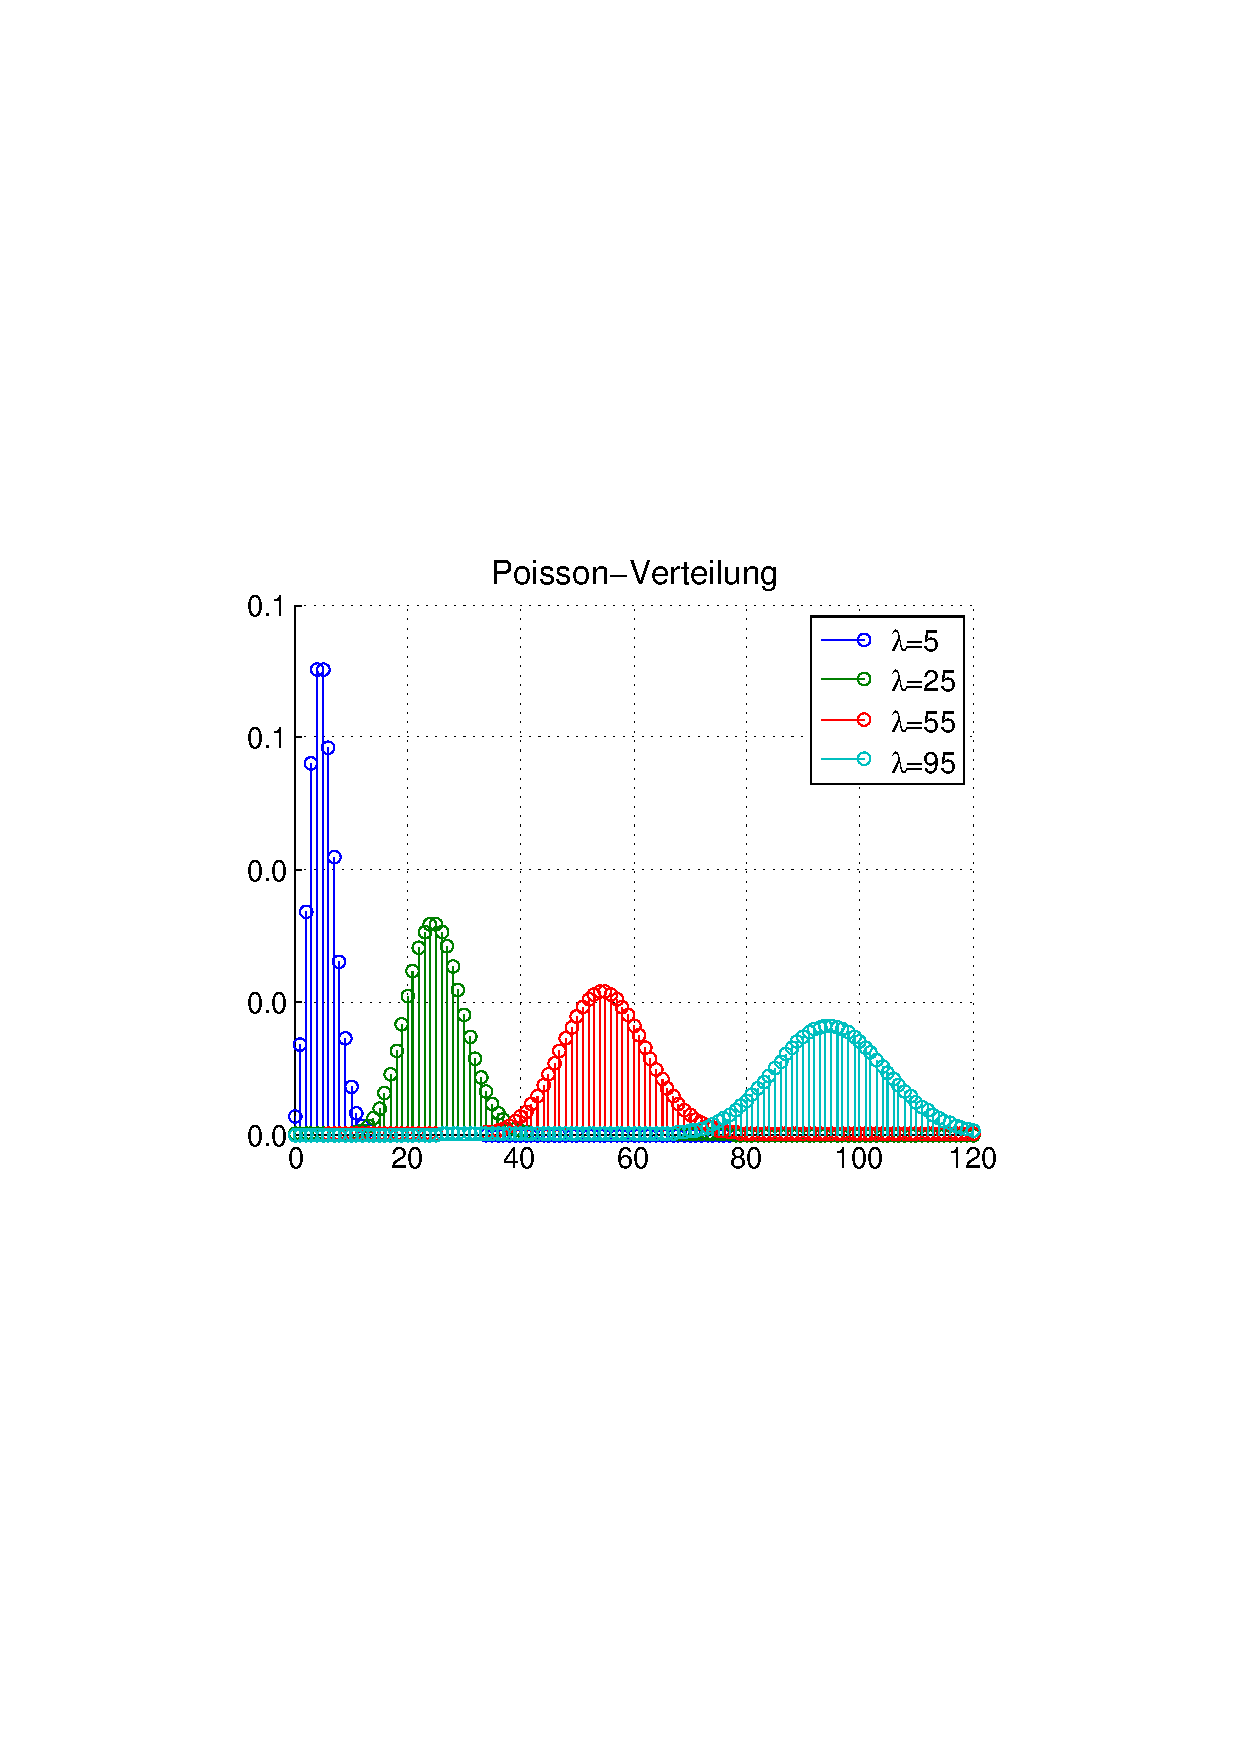
\includegraphics[width=10cm,trim=4.0cm 9.5cm 4.0cm 9.25cm ,clip]{Content/RandomVariable/Poisson}

\vspace{2mm}
\hrule
\vspace{3mm}

\subsubsection{Geometric RV $X\sim Geom(p)$}

\begin{minipage}{10cm}
	\begin{liste}
		\item Number of independent trials required until first success
		\vspace{0.2cm}
		\item $\boxed{p(\{X=i\}) = (1-p)^{i-1}p\qquad i=\{1,2,\ldots\}}$
	\end{liste}
\end{minipage}
\hfill
\begin{minipage}{8cm}
	\begin{liste}
		\item $E(X)=\frac 1p$
		\item $Var(X)=\frac {1-p}{p^2}$
		\item $\phi(t)=\frac{p\e^t}{1-(1-p)\e^t}$
	\end{liste}
\end{minipage}
\hfill

\vspace{2mm}
\hrule
\vspace{3mm}

\subsection{Continuous Random Variables \skript{34}}
\subsubsection{Uniform RV $X\sim U(\alpha,\beta)$ \skript{34}}
\begin{minipage}{10cm}
$f_X(x) = \twopartdef { \frac{1}{\beta-\alpha} } {\alpha \leq x \leq\beta} {0} {\text{otherwise}}$
\end{minipage}
\begin{minipage}{10cm}
	\begin{liste}
		\item $E(X)=\frac {\alpha+\beta}{2}$
		\item $Var(X)=\frac {(\alpha-\beta)^2}{12}$
		\item $\phi(t)=\frac{\e^{t\beta}-\e^{t\alpha}}{t(\beta-\alpha)}$
	\end{liste}
\end{minipage}
\hfill
\vspace{2mm}
\hrule
\vspace{3mm}

\subsubsection{Exponential RV $X\sim Exp(\lambda)$ \skript{35}}
\begin{minipage}{10cm}

\begin{equation}
f_X(x) = \twopartdef { \lambda\e^{-\lambda x} } {x\geq 0} {0} {x<0}\\
F_X(x) = \twopartdef { 1-\e^{-\lambda x} } {x\geq 0} {0} {x<0}\nonumber
\end{equation}

\end{minipage}
\begin{minipage}{9cm}
	\begin{liste}
		\item $E(X)=\frac {1}{\lambda}$
		\item $Var(X)=\frac {1}{\lambda^2}$
		\item $\phi(t)=\frac{\lambda}{\lambda-t}$
		\item $\max(f_X)$ when $f_X(0)=\lambda$
		\item $P[X>s+t | X>t]= \displaystyle\frac{ \e^{-\lambda (s+t)} }{ \e^{-\lambda t} }=\e^{-\lambda s} = P[X>s]$
	\end{liste}
\end{minipage}
\hfill

\vspace{2mm}
\hrule
\vspace{3mm}

\subsubsection{Normal RV $X\sim N(\mu,\sigma^2)$ \skript{36-39}}
\begin{minipage}{10cm}
$f_X(x) = \displaystyle\frac{1}{\sqrt{2\pi}\sigma}\cdot\e^{\displaystyle\frac{-(x-\mu)^2}{2\sigma^2}}\qquad -\infty <x<\infty$
\end{minipage}
\begin{minipage}{10cm}
	\begin{liste}
		\item $E(X)=\mu$
		\item $Var(X)=\sigma^2$
		\item $\phi(t)=\e^{\frac{\sigma^2t^2}{2}+\mu t}$
	\end{liste}
\end{minipage}
\hfill

\textbf{Example:}\\
If $X\sim N(\mu,\sigma^2)$ and $Y=\alpha X+ \beta$, \qquad
then: $Y\sim N(\alpha\mu+\beta,\alpha^2\sigma^2)$\\



\subsubsection{Standard normal distribution $\Phi(x)$:}

\textbf{Normalisation:} $Y=\frac{X-\mu}{\sigma}\sim N(0,1)$ \qquad for \qquad $X\sim N(\mu,\sigma^2)$ \qquad $\Rightarrow$ \qquad
$\underbrace{\Phi(x)=\displaystyle\frac 1 {\sqrt{2\pi}}\int\limits_{-\infty}^x{\displaystyle\e^{\displaystyle\frac{-y^2}{2}}dy} }_{\text{cumulative distribution function}}$\\

\vspace{0.5cm}

\textbf{Example:} $X\sim N\big(\mu,\sigma^2\big)\quad \Rightarrow \quad P\big(\alpha<X<\beta\big)\quad\overset{Norm.}{=}\quad P\big(\frac{\alpha-\mu}{\sigma}<\frac{X-\mu}{\sigma}<\frac{\beta-\mu}{\sigma}\big)=\underbrace{\Phi\left(\frac{\beta-\mu}{\sigma}\right)-\Phi\left(\frac{\alpha-\mu}{\sigma}\right)}\limits_{\text{Std.-Normal-Distr. table}}$\\
\textbf{Bei negativen Werten:} $\boxed{\Phi(\alpha)=1-\Phi(-\alpha)}$


\vspace{2mm}
\hrule

\subsubsection{Bivariate Normal RV }

$f_{X1,X2}(x1,x2)=\displaystyle\frac{1}{2\pi\sigma_1\sigma_2\sqrt{1-\rho^2}}\cdot\e^{\displaystyle-\frac{1}{2(1-\rho^2)}\left[\left(\frac{x_1-\mu_1}{\sigma_1}\right)^2-2\rho\frac{x_1-\mu_1}{\sigma_1}\frac{x_2-\mu_2}{\sigma_2}+\left(\frac{x_2-\mu_2}{\sigma_2}\right)^2\right]}$\\

$f_{X_1|X_2}(x_1|x_2)=\displaystyle\frac{1}{\sqrt{2\pi}\cdot \sigma_1}\frac{1}{\sqrt{1-\rho^2}}\cdot\e^{\displaystyle-\frac{\left(x_1-\mu_1-\rho\frac{\sigma_1}{\sigma_2}(x_2-\mu_2)\right)^2}{2(1-\rho^2)\sigma_1^2}}$\\

$E(X_1|X_2=x_2)=\mu_1+\rho\frac{\sigma_1}{\sigma_2}(x_2-\mu_2)$ (see example 18, \formelbuch{52})\\
$Var(X_1|X_2=x_2)=\sigma_1^2(1-\rho^2)$

\vspace{2mm}
\hrule

\subsubsection{Multivariate Normal RV $\mathbf{X} \sim N(\mathbf{\mu},\mathbf{C})$}
$f_X(x)=\displaystyle\frac{1}{(2\pi)^{n/2}\sqrt{det(C)}}\cdot\e^{\displaystyle-\frac{1}{2}(x-\mu)^T\cdot C^{-1}\cdot(x-\mu)}$\\
$E(X_i)=\mu_i$\\
$Var(X_i)=\sum\limits_{j=i}^n{a_{ij}^2=C_{ii}}$\\
$\phi_X(t_1,\ldots,t_m)=E(\e^{t_1X_1+\ldots+t_mX_m})$

\vspace{2mm}
\hrule
